\documentclass{article}
\usepackage[english]{babel}
\usepackage[utf8]{inputenc}
\usepackage{graphicx}
\usepackage{titletoc}
\usepackage[section]{placeins}
\usepackage{siunitx}
\usepackage{amsmath}
\usepackage{caption}
\usepackage{fancyhdr}
\usepackage{tabto}
\usepackage{listings}

\pagestyle{fancy}
\fancyhf{}
\rhead{Schäfer, Schnöll}
\lhead{EPH Labor}
\rfoot{Seite \thepage}

\begin{document}

\tableofcontents

\section{Inventarliste}
  \begin{itemize}
    \item Raspberry Pi 3
    \item Potentiometer Rx 10k \si{\ohm}
    \item MCP3008 (Analog-Digital Converter)
    \item Widerstand R1 1000 \si{\ohm}
  \end{itemize}

\newpage
\section{Strom- / Spannungsmessung und Verlauf aufnehmen mittels Raspberry Pi}
In dieser Laborübung ging es um die Aufnahme von analogen Signalen mit dem Raspberry Pi und die digitale Verarbeitung. 
Als analoge Signale dienen einerseits ein Spannungsabfall über einem Potentiometer sowie die Lade\- und Entladekurve eines Kondensators.

\subsection{Vorbereitung}
Als Vorbereitung für das Labor wurde der Raspberry Pi konfiguriert und ein Programm für die Behandlung der digitalen Inputs erstellt.
Weiteres wurde das Datenblatt für den Analog-Digital Converter (fortfolgend ADC) MCP3008 heruntergeladen. Die Pinbelegung ist im nachfolgenden Bild~\ref{fig:ADCPinbelegung} ersichtlich.

\begin{figure}[h!]
    \centering
    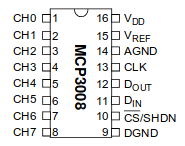
\includegraphics[width=0.4\textwidth]{MCP3008-Pinbelegung.png}
    \caption{Pinbelegung MCP3008}
    \label{fig:ADCPinbelegung}
\end{figure}

\newpage
\subsection{ADC an den Raspberry Pi anschließen}
Der MCP3008 ermöglicht die Verarbeitung von acht analogen Signalen, diese können an die linke Seite des ADC angeschlossen werden.
Auf der Seite des Raspberry Pis muss die Hardware SPI Schnittstelle aktiviert werden. Danach ist es möglich mittels der \textit{wiringPi.h} Library die Schnittstelle anzusteuern.
Die Verkabelung ist in Bild~\ref{fig:ADC-Verkabelung} visualisiert.

\begin{figure}[h!]
    \centering
    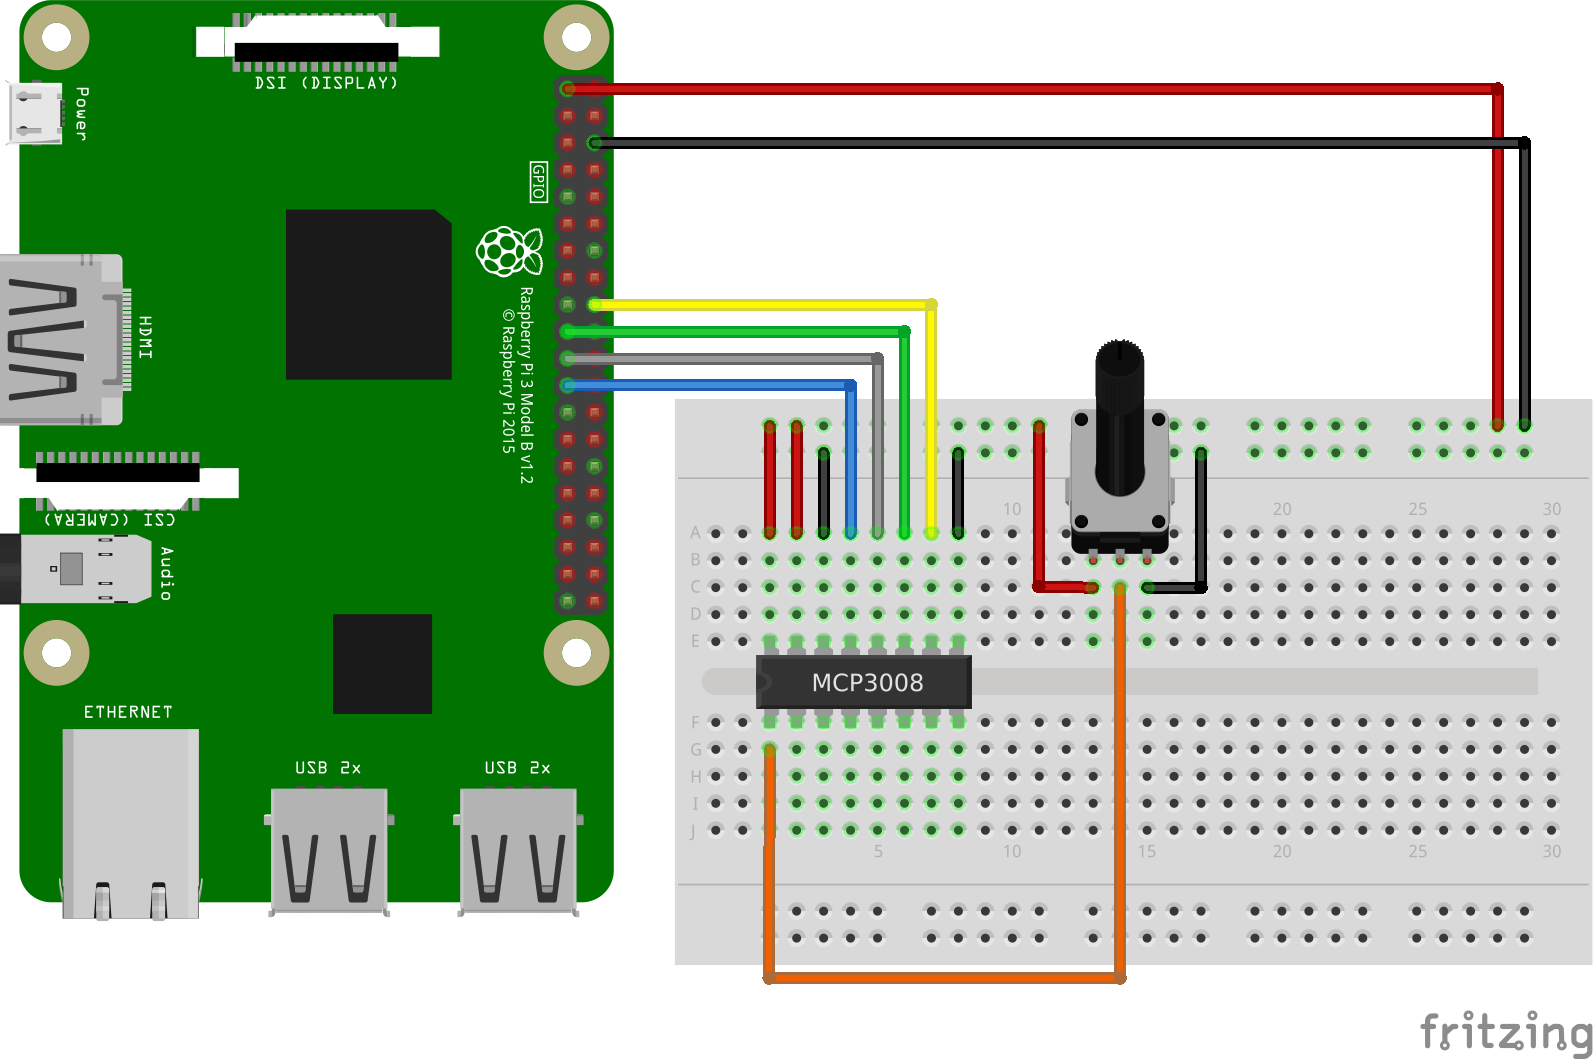
\includegraphics[width=0.8\textwidth]{RPi-Fritzing-Potentiometer_bb.png}
    \caption{Verkabelung mit dem Raspberry Pi}
    \label{fig:ADC-Verkabelung}
\end{figure}

Die Pin Verkabelung des Raspberry Pis mit dem MCP3008 wird in nachstehender Tabelle \ref{tab:Verkabelung} dargestellt. 
\begin{table}[h!]
    \begin{tabular}{|l|l|l|l|l|}
    \hline
    \multicolumn{2}{|l|}{\textbf{MCP3008}} & \multicolumn{2}{l|}{\textbf{Raspberry Pi}} & \textbf{Bemerkung}         \\ \hline
    Pin         & Signal          & Pin         & Signal              &                            \\ \hline
    16          & VDD             & 1           & 3v3                 &                            \\ \hline
    15          & VREF            & 1           & 3v3                 &                            \\ \hline
    14          & AGND            & 6           & GND                 &                            \\ \hline
    13          & CLK             & 23          & SCLK                & Clock Synchronization      \\ \hline
    12          & DOUT            & 21          & GPIO9 MISO          & Master-In Slave-Out        \\ \hline
    11          & DIN             & 19          & GPIO10 MOSI         & Master-Out Slave-In        \\ \hline
    10          & CS/SHDN         & 24          & GPIO24 CE0          & Chip Enable (Slave Select) \\ \hline
    9           & DGND            & 6           & GND                 &                            \\ \hline
    \end{tabular}
    \caption{Pin Mapping}
    \label{tab:Verkabelung}
\end{table}

\newpage
\subsubsection{Kontrollfragen}

\textbf{Was macht ein ADC? Für was wird er verwendet?}
\begin{itemize}
    \item sehr kluge Antwort
\end{itemize}
\textbf{Finden Sie die wichtigsten Kenngrößen des verwendeten ADCS MCP3004/3008 heraus.}
\begin{itemize}
    \item sehr kluge Antwort
\end{itemize}
\textbf{Was sind die Channels am ADC?}
\begin{itemize}
    \item sehr kluge Antwort
\end{itemize}
\textbf{Was ist eine SPI Schnittstelle?}
\begin{itemize}
    \item sehr kluge Antwort
\end{itemize}
\textbf{Wie funktioniert die SPI Schnittstelle?}
\begin{itemize}
    \item sehr kluge Antwort
\end{itemize}
\textbf{Was ist ein Channel (Kommunikation, zb. SPI-Channel)}
\begin{itemize}
    \item sehr kluge Antwort
\end{itemize}

\newpage

\subsection{Spannungsmessung mit ADC und Potentiometer}
Die Verkablung mit dem Potentiometer wurde abgeschlossen, als nächstes wurde ein Programm entwickelt, welche die SPI Schnittstelle anspricht und die ausgelesenen Werte neben der Ausgabe in der Konsole, zusätzlich in eine Datei abspeichert.
Das Auslesen der SPI Schnittstelle erfolgt mittels der Funktion \textit{int analogRead()}. \\
Die Funktion \textit{int saveSPI(int amount, int interval, char filename[])} ermöglicht es einen Zeitintervall, die Anzahl der zu lesenden Inputs und einen Dateinamen als Parameter zu übergeben.
Die gelesen Signale werden in folgenden Format nun in eine Log-Datei geschrieben:

\begin{lstlisting}
Counter Value
    0	4
    1	19
    2	26
    3	32
    4	39
    5	45
    6	52
    7	58
    8	64
    9	71
    10	77
    11	83
    12	87
    13	94
    14	100
    15	105
    16	111
\end{lstlisting}

\subsubsection{Visualiserung mittels \textit{gnuplot}}



\subsubsection{Kontrollfragen}

\textbf{In welchen Bereich bewegen sich die Werte? Warum ist das so?}
\begin{itemize}
    \item sehr kluge Antwort
\end{itemize}
\textbf{Stellen Sie eine Formel für die Umrechnung des ADC-Wertes in einen Spannungswert auf.}
\begin{itemize}
    \item sehr kluge Antwort
\end{itemize}


\newpage
\listoffigures

\listoftables

\end{document}